% generated by make_combined.py from stage4_causal_checks/stage4.tex; do not edit
\section{Stage 4 --- Is it location, or which images carry the artifact?}\label{sec:stage4}

\stagebox{\textbf{In one sentence.} The images whose artifact lies inside the ROI differ strongly from those whose
artifact lies outside it (standardised differences up to \sFourSmdBeforeCap), but the real-artifact crossover survives
covariate matching and doubly robust regression adjustment in all three cohorts where matching is feasible
(\sFourNATwoOK{} of \sFourNATwo); pasting the same real artifact inside or outside the ROI of the same images reproduces
the location effect, although a neutral paste of the same shape reproduces most of it, so only a smaller part ---
significant for hair and thyroid calipers --- is attributable to the artifact's content; the crossover is also robust
to the artifact-label definition, to stricter leakage groups and to a full rebuild of the data on a second machine.}
\subsection{Where this stage starts}
Stage~3 showed a positive crossover with real artifacts in four cohorts and three encoder families. Its design compares
two different sets of images: those whose artifact happens to lie inside the ROI (Trap~A) and those whose artifact lies
outside it (Trap~B). Real artifacts are not placed at random. In dermoscopy, hair lies on large lesions more often than on
small ones; in thyroid ultrasound, calipers inside the nodule are drawn on larger, more heavily measured nodules.
Artifact-debiasing studies in dermoscopy make the same point \citep{bissoto2020debiasing,nauta2022uncovering}. The
crossover could therefore reflect \emph{which images} carry in-ROI artifacts rather than \emph{where} the artifact lies.
This stage separates the two, and then tests how fragile the result is to the choices that define it.

\subsection{Questions}
\begin{enumerate}[label=\textbf{Q4\alph*},leftmargin=*]\itemsep1pt
\item Do Trap-A and Trap-B images differ, and is the crossover explained by measured differences between them?
\item Does the location effect survive when the artifact is moved within the \emph{same} image --- and how much of that
is due to the artifact rather than to pasting something into the image?
\item Is the crossover robust to how the artifact label is defined, to stricter leakage groups, and to rebuilding the
whole pipeline?
\end{enumerate}
\paragraph{Why three causal checks} Matching removes measured imbalance but depends on the chosen covariates;
regression on the matched sample (a doubly robust combination) protects against residual imbalance and against
misspecification of either step alone; transplantation removes image-level confounding altogether but introduces its
own artifact --- the paste. The neutral paste (same mask shape, same compositing, filled with artifact-free tissue from
the donor) measures that paste effect. \emph{Rejected alternatives}: inverse-probability weighting (standardised
differences above 2 in dermoscopy and capsule give extreme weights) and synthetic control images (they would repeat
Stage~2, not test real artifacts).

\subsection{Methods}
\paragraph{Balance and matching (R1)} Covariates fixed before any matching: dermoscopy --- lesion area, hair amount,
age, sex, body site, source, diagnosis within label; thyroid --- nodule area, caliper pixels (log), native width and
height (scanner proxy), mean grey level (gain proxy), nodule depth; ovary --- tumour area, caliper pixels, image size,
grey level, subtype within label; capsule --- lesion-box area, contamination fraction, brightness, frame block (acquisition
proxy). Standardised mean differences between the Trap-A and Trap-B artifact images, within label and pooled. Greedy
1:1 nearest-neighbour matching on the logit of a propensity model within label (exactly within source for dermoscopy),
without replacement, calliper 0.2 SD; 0.05 SD as a stricter sensitivity analysis (R7). A cohort with fewer than 30
matched images per label is infeasible. The matched images replace the artifact cells of the traps; everything else is
unchanged.
\paragraph{Regression adjustment (A2)} For each reversed-test image of the matched sample, the \emph{placement value} of
the masked minus the ERM score (for a positive: the weighted share of negatives ranked below it; for a negative: the
complement of the share of positives ranked above it), so that the class means reproduce the AUROC and the unadjusted
difference between traps equals the crossover exactly (verified per seed). Within each seed, weighted least squares of
this outcome on an intercept, the Trap-B indicator, the label and all matching covariates; the adjusted crossover is the
Trap-B coefficient averaged over seeds. Crossed bootstrap with placement values and regression recomputed in every
replicate (2,000 replicates); Holm over the three cohorts.
\paragraph{Transplant (R2) and neutral paste (R5)} For each artifact-free recipient image, a real artifact instance is cut
from a donor image of the same cohort (the donor's mask pixels, largest connected component) and alpha-composited at a
position fully inside ($\ge95\%$ overlap) and at a position fully outside (0\%) the recipient's ROI, with a random dihedral
transform; the positions are restricted to the field of view. The environments are then built as in the controlled sweeps
with the pasted instance as the artifact; 5 presence seeds $\times$ 5 grouped folds. The neutral paste keeps the mask
shape, transform, positions and compositing but fills the mask with tissue from the donor image at a window that does not
touch its artifact.
\paragraph{Robustness} (i) Artifact-label definitions: large detections only ($\ge50$ caliper pixels) and strict location
($r\ge0.7$ / $r<0.05$) for thyroid and ovary; for capsule, a Trap~B that also requires debris to cover less than 5\% of the
lesion box. (ii) Leakage: embedding-based near-duplicate groups (below). (iii) Rebuild: every dataset re-downloaded and
every derived object --- lesion U-Net, caliper detector, debris probe, leakage groups, feature caches --- rebuilt on a
second machine.

\subsection{Experiments}
\begin{table}[H]\centering\scriptsize
\caption{Experiments of this stage and their registration documents (\texttt{docs/PREREGISTRATION\_<name>.md} or \texttt{docs/<name>.md}). Commit times are set by the committing machine and are not independent proof of order; the REVIEW2, REVIEW3 and FINAL registrations were also pushed to GitHub before their runs.}\label{s4:tab:exp}
\begin{tabular}{p{3.1cm}p{2.1cm}p{2.4cm}p{3.2cm}p{3.3cm}}\toprule
Experiment & Status & Registration & First commit (local time) & Support criterion \\\midrule
Covariate balance (SMD) and matched traps, M1 & \ok{} registered & REVIEW2 (R1) & \texttt{29cd0da}, 2026-09-27 18:56 & matched crossover CI $>0$, Holm over 3 feasible cohorts \\
Stricter calliper 0.05 SD (R7) & \ok{} registered & REVIEW3 & \texttt{85da735}, 2026-09-27 23:43 & sensitivity, descriptive \\
Real-artifact transplant, T1 & \ok{} registered & REVIEW2 (R2) & \texttt{29cd0da}, 2026-09-27 18:56 & interaction CI $>0$, Holm over 4 \\
Neutral paste (paste-edge control), N3 & \ok{} registered & REVIEW3 (R5) & \texttt{85da735}, 2026-09-27 23:43 & artifact $-$ neutral interaction CI $>0$ \\
Regression-adjusted crossover, A2 & \ok{} registered & FINAL (A2) & \texttt{c45d482}, 2026-09-28 00:35 & adjusted crossover CI $>0$, Holm over 3 \\
Artifact-label sensitivity & \ok{} registered & SENSITIVITY\_\allowbreak{}ARTIFACT\_\allowbreak{}LABELS & \texttt{c1bdfdf}, 2026-09-27 09:46 & crossover keeps sign and CI $>0$ in every variant \\
Embedding-based leakage groups & \ok{} registered & EMBEDDING\_\allowbreak{}GROUPS & \texttt{b0eda23}, 2026-09-27 13:55 & same sign and CI verdict as with pHash groups \\
Rebuild on a second machine, R0 & \ok{} registered & REVIEW2 (R0) & \texttt{29cd0da}, 2026-09-27 18:56 & same sign, CI $>0$, $|\Delta|\le0.03$ \\
Capsule matched analysis & \no{} descriptive & REVIEW2 (R1) & \texttt{29cd0da}, 2026-09-27 18:56 & infeasible under the registered rule \\
\bottomrule\end{tabular}
\end{table}


\subsection{Results}
\subsubsection{The traps contain different images}
The in-ROI and out-of-ROI artifact images differ strongly (Table~\ref{s4:tab:bal}): in dermoscopy the largest SMD is
\sFourSmdBeforeHair{} (\sFourWorstHair: hair lies inside large lesions), in capsule \sFourSmdBeforeCap{} (\sFourWorstCap),
in thyroid \sFourSmdBeforeThy{} (\sFourWorstThy) and in ovary \sFourSmdBeforeOv. Stage~3's crossover is therefore not a
comparison of like with like.
\begin{table}[H]\centering\scriptsize
\caption{Balance of pre-specified covariates between the in-ROI (Trap~A) and out-of-ROI (Trap~B) artifact images, before and after 1:1 nearest-neighbour matching within label (calliper 0.2 SD, pooled standardised mean differences). Registered rule: fewer than 30 matched images per label in either trap makes a cohort infeasible; target max $|$SMD$|\le0.1$ after matching.}\label{s4:tab:bal}
\resizebox{\linewidth}{!}{\begin{tabular}{lccccc}\toprule
Cohort & Least balanced covariate & max $|$SMD$|$ before & after matching & min matched pairs per label & feasible (rule) \\\midrule
ISIC hair & lesion\_area & 2.127 & 0.108 & 398 & yes \\
Thyroid & caliper\_px\_log & 0.527 & 0.045 & 93 & yes \\
Ovary & caliper\_px\_log & 0.389 & 0.079 & 86 & yes \\
Capsule & roi\_area & 2.574 & 0.231 & 19 & \textbf{no} \\
\bottomrule\end{tabular}}
\end{table}

\begin{table}[H]\centering\scriptsize
\caption{Per-covariate balance, thyroid and ovary (pooled over labels). The dermoscopy and capsule tables (17 and 20 covariates) are in \texttt{results/rerun\_2026-09-28/review2/R1\_balance.csv}.}\label{s4:tab:baldet}
\begin{tabular}{lccc}\toprule
Cohort & Covariate & SMD before & SMD after \\\midrule
Thyroid & roi\_area & $+0.395$ & \na \\
Thyroid & caliper\_px\_log & $+0.527$ & \na \\
Thyroid & width & $-0.143$ & \na \\
Thyroid & height & $-0.123$ & \na \\
Thyroid & mean\_grey & $+0.183$ & \na \\
Thyroid & roi\_centroid\_row & $+0.060$ & \na \\
Ovary & roi\_area & $+0.320$ & \na \\
Ovary & caliper\_px\_log & $+0.389$ & \na \\
Ovary & width & $-0.298$ & \na \\
Ovary & height & $+0.047$ & \na \\
Ovary & mean\_grey & $+0.107$ & \na \\
Ovary & subtype=0.0 & $+0.149$ & $-0.079$ \\
Ovary & subtype=1.0 & $+0.059$ & $+0.072$ \\
Ovary & subtype=2.0 & $-0.159$ & $-0.012$ \\
Ovary & subtype=3.0 & $-0.054$ & $+0.000$ \\
Ovary & subtype=4.0 & $-0.022$ & $+0.024$ \\
Ovary & subtype=6.0 & $+0.024$ & $+0.056$ \\
Ovary & subtype=7.0 & $-0.020$ & $-0.062$ \\
\bottomrule\end{tabular}
\end{table}


\subsubsection{Matching}
Matching brings the maximum pooled SMD to \sFourSmdAfterHair{} (dermoscopy), \sFourSmdAfterThy{} (thyroid) and
\sFourSmdAfterOv{} (ovary); capsule matching is infeasible (\sFourPairsCap{} pairs in the smaller label; SMD after matching
\sFourSmdAfterCap). The crossover is essentially unchanged (Table~\ref{s4:tab:match}): dermoscopy \sFourMatchHair, thyroid
\sFourMatchThy, ovary \sFourMatchOv{} (M1 supported in all three after Holm); with the stricter calliper it shrinks by
9--16\% and survives: \sFourMatchFiveHair, \sFourMatchFiveThy, \sFourMatchFiveOv. Capsule, matched descriptively, gives
\sFourMatchCap{} --- lower than unmatched (\sFourXCap) and imprecise, so capsule's real-trap crossover is reported as
descriptive.
\begin{table}[H]\centering\scriptsize
\caption{Crossover before and after covariate matching (reversed-test AUROC, crossed 95\% CIs). The 0.05 SD calliper is a stricter, registered sensitivity analysis (R7).}\label{s4:tab:match}
\resizebox{\linewidth}{!}{\begin{tabular}{lcccc}\toprule
Cohort & Crossover, all images & matched (0.2 SD) & matched (0.05 SD) & M1 (Holm, 3) \\\midrule
ISIC hair & $+0.147$ [$+0.111, +0.185$] & $+0.154$ [$+0.123, +0.186$] & $+0.124$ [$+0.086, +0.162$] & \ok \\
Thyroid & $+0.239$ [$+0.196, +0.280$] & $+0.238$ [$+0.186, +0.290$] & $+0.218$ [$+0.165, +0.270$] & \ok \\
Ovary & $+0.170$ [$+0.087, +0.252$] & $+0.163$ [$+0.050, +0.273$] & $+0.152$ [$+0.041, +0.265$] & \ok \\
Capsule & $+0.377$ [$+0.327, +0.426$] & $+0.230$ [$+0.036, +0.434$] & $+0.328$ [$+0.087, +0.573$] & descriptive (infeasible) \\
\bottomrule\end{tabular}}
\end{table}


\subsubsection{Regression adjustment on the matched sample (A2)}
Within-label imbalance up to about 0.16 remained after matching. The doubly robust adjusted crossover equals the
unadjusted one to the third decimal in every cohort (Table~\ref{s4:tab:a2}): dermoscopy \sFourAdjHair{} (unadjusted
\sFourUnadjHair), thyroid \sFourAdjThy{} (\sFourUnadjThy), ovary \sFourAdjOv{} (\sFourUnadjOv); Holm-adjusted $p$ =
\sFourAdjHolmHair, \sFourAdjHolmThy{} and \sFourAdjHolmOv. All \sFourNATwo{} registered tests are supported. Residual
measured imbalance does not carry the effect. What this cannot exclude is an \emph{unmeasured} difference.
\begin{table}[H]\centering\scriptsize
\caption{Regression-adjusted crossover on the matched traps (A2): per-image placement values of the masked minus the ERM score regressed on the Trap-B indicator, the label and all matching covariates, within seed; crossed bootstrap (2,000 replicates). Capsule is not analysed (matching infeasible; descriptive only).}\label{s4:tab:a2}
\resizebox{\linewidth}{!}{\begin{tabular}{lccccccc}\toprule
Cohort & Test images per seed & Covariate columns & Post-matching max $|$SMD$|$ pooled / per label & Unadjusted crossover & Adjusted (doubly robust) & $p$ (Holm, 3) & A2 \\\midrule
ISIC hair & 2960 & 17 & 0.108 / 0.164 & $+0.154$ [$+0.124, +0.186$] & $+0.156$ [$+0.127, +0.187$] & 0.002 & \ok \\
Thyroid & 2150 & 6 & 0.045 / 0.150 & $+0.238$ [$+0.185, +0.291$] & $+0.238$ [$+0.184, +0.291$] & 0.002 & \ok \\
Ovary & 576 & 11 & 0.079 / 0.140 & $+0.163$ [$+0.058, +0.268$] & $+0.165$ [$+0.056, +0.273$] & 0.002 & \ok \\
\bottomrule\end{tabular}}
\end{table}

\begin{table}[H]\centering\scriptsize
\caption{Post-matching balance table of the A2 sample (pooled over labels; test images of the reversed environment).}\label{s4:tab:a2bal}
\begin{tabular}{lcccc}\toprule
Cohort & Covariate & Trap A mean & Trap B mean & SMD \\\midrule
ISIC hair & lesion\_area & 0.297 & 0.292 & $+0.033$ \\
ISIC hair & hair\_amount & 0.018 & 0.015 & $+0.108$ \\
ISIC hair & age & 57.119 & 57.332 & $-0.012$ \\
ISIC hair & age\_missing & 0.019 & 0.026 & $-0.048$ \\
ISIC hair & sex=female & 0.504 & 0.521 & $-0.035$ \\
ISIC hair & sex=male & 0.480 & 0.457 & $+0.046$ \\
ISIC hair & sex=missing & 0.016 & 0.022 & $-0.040$ \\
ISIC hair & site=head/neck & 0.174 & 0.179 & $-0.013$ \\
ISIC hair & site=lower extremity & 0.219 & 0.213 & $+0.015$ \\
ISIC hair & site=missing & 0.076 & 0.072 & $+0.015$ \\
ISIC hair & site=oral/genital & 0.001 & 0.002 & $-0.015$ \\
ISIC hair & site=palms/soles & 0.027 & 0.030 & $-0.020$ \\
ISIC hair & site=torso & 0.383 & 0.387 & $-0.008$ \\
ISIC hair & site=upper extremity & 0.120 & 0.118 & $+0.008$ \\
ISIC hair & benign\_dx=BKL & 0.092 & 0.100 & $-0.026$ \\
ISIC hair & benign\_dx=MEL & 0.218 & 0.218 & $+0.000$ \\
ISIC hair & benign\_dx=NV & 0.442 & 0.413 & $+0.060$ \\
ISIC hair & benign\_dx=other & 0.248 & 0.270 & $-0.050$ \\
ISIC hair & source=BCN & 0.545 & 0.545 & $+0.000$ \\
ISIC hair & source=HAM & 0.386 & 0.386 & $+0.000$ \\
ISIC hair & source=MSK & 0.069 & 0.069 & $+0.000$ \\
Thyroid & roi\_area & 0.117 & 0.118 & $-0.008$ \\
Thyroid & caliper\_px\_log & 5.495 & 5.448 & $+0.037$ \\
Thyroid & width & 450.288 & 441.291 & $+0.045$ \\
Thyroid & height & 373.576 & 371.744 & $+0.017$ \\
Thyroid & mean\_grey & 60.457 & 60.609 & $-0.006$ \\
Thyroid & roi\_centroid\_row & 0.367 & 0.366 & $+0.007$ \\
Ovary & roi\_area & 0.141 & 0.142 & $-0.001$ \\
Ovary & caliper\_px\_log & 6.518 & 6.481 & $+0.032$ \\
Ovary & width & 864.648 & 856.939 & $+0.037$ \\
Ovary & height & 550.073 & 549.944 & $+0.003$ \\
Ovary & mean\_grey & 57.307 & 56.935 & $+0.022$ \\
Ovary & subtype=0.0 & 0.218 & 0.251 & $-0.079$ \\
Ovary & subtype=1.0 & 0.201 & 0.173 & $+0.072$ \\
Ovary & subtype=2.0 & 0.296 & 0.302 & $-0.012$ \\
Ovary & subtype=3.0 & 0.089 & 0.089 & $+0.000$ \\
Ovary & subtype=4.0 & 0.061 & 0.056 & $+0.024$ \\
Ovary & subtype=6.0 & 0.106 & 0.089 & $+0.056$ \\
Ovary & subtype=7.0 & 0.028 & 0.039 & $-0.062$ \\
\bottomrule\end{tabular}
\end{table}


\subsubsection{The same artifact inside and outside the ROI}
\begin{figure}[H]\centering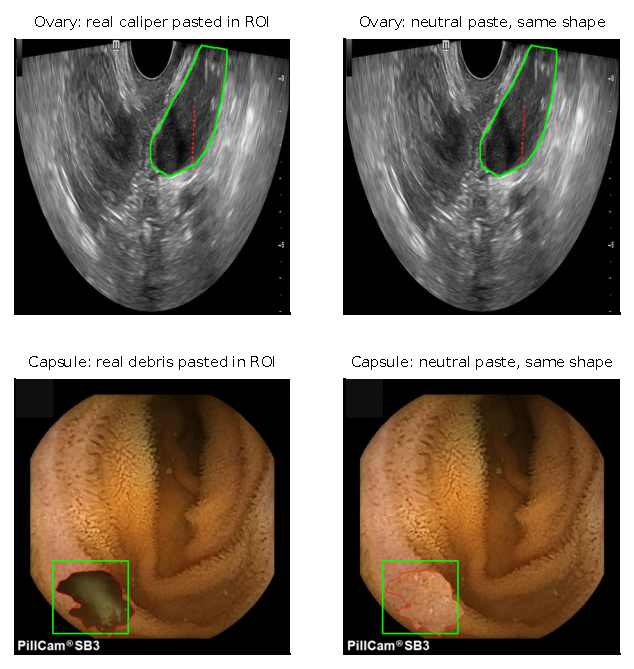
\includegraphics[width=0.60\linewidth]{../stage4_causal_checks/figures/transplant_examples.pdf}
\caption{Transplant and neutral paste on the same recipient images (openly licensed cohorts; MMOTU, SEE-AI CC BY 4.0).
Left: a real artifact instance pasted inside the ROI (\textcolor{roigreen}{green}; the pasted region outlined in
\textcolor{artred}{red}). Right: the neutral paste --- same mask shape and compositing, filled with artifact-free tissue
from the donor.}\label{s4:fig:tx}\end{figure}
Pasting the same real instance outside versus inside the ROI yields a positive location interaction in every cohort
(Table~\ref{s4:tab:tx}; dermoscopy \sFourTIHair, thyroid \sFourTIThy, ovary \sFourTIOv, capsule \sFourTICap; Holm over four).
Table~\ref{s4:tab:txdet} shows the mechanism of Stage~2 on real artifacts: outside the ROI masking removes the pasted
artifact completely --- the masked model's correlated and reversed AUROC coincide (e.g.\ thyroid \sFourMaskCorrOutThy{}
and \sFourMaskRevOutThy) and $|\Delta p|=0$ --- whereas inside it the artifact survives, and for thyroid, ovary and capsule
the masked model reacts to it \emph{more} than ERM (capsule \sFourDpMaskInCap{} versus \sFourDpErmInCap). Group balancing
has a small location interaction of the opposite sign (e.g.\ \sFourTBalHair{} for hair), much smaller than
masking's: it is nearly location-invariant.
\begin{table}[H]\centering\scriptsize
\caption{Real-artifact transplant (T1): the same real artifact instance, cut from a donor image, pasted outside and inside the ROI of the same artifact-free recipient images. These effects combine the artifact with the paste itself (seam, occluded tissue); Table~\ref{s4:tab:neutral} separates them.}\label{s4:tab:tx}
\resizebox{\linewidth}{!}{\begin{tabular}{lcccc}\toprule
Cohort & mask $-$ ERM, pasted outside ROI & pasted inside ROI & Location interaction & Balanced: interaction \\\midrule
ISIC hair & $+0.178$ [$+0.128, +0.227$] & $-0.075$ [$-0.114, -0.036$] & $+0.253$ [$+0.214, +0.293$] & $-0.052$ [$-0.071, -0.033$] \\
Thyroid & $+0.349$ [$+0.321, +0.379$] & $+0.072$ [$+0.043, +0.100$] & $+0.277$ [$+0.256, +0.298$] & $-0.016$ [$-0.025, -0.007$] \\
Ovary & $+0.064$ [$+0.001, +0.126$] & $-0.010$ [$-0.075, +0.056$] & $+0.074$ [$+0.044, +0.104$] & $-0.011$ [$-0.025, +0.002$] \\
Capsule & $+0.322$ [$+0.262, +0.384$] & $-0.175$ [$-0.241, -0.109$] & $+0.497$ [$+0.427, +0.567$] & $-0.032$ [$-0.068, +0.004$] \\
\bottomrule\end{tabular}}
\end{table}

\begin{table}[H]\centering\scriptsize
\caption{Transplant, per location: correlated and reversed AUROC of ERM and of the masked model, and the same-head counterfactual sensitivity to the pasted artifact (T3). Outside the ROI the masked model's correlated and reversed AUROC coincide and $|\Delta p|=0$: the pasted artifact is gone.}\label{s4:tab:txdet}
\resizebox{\linewidth}{!}{\begin{tabular}{lcccccc}\toprule
Cohort & Recipients & ERM in: corr / rev & mask in: corr / rev & mask out: corr / rev & $|\Delta p|$ in: ERM / mask & $|\Delta p|$ out: mask \\\midrule
ISIC hair & 860 & 0.904 / 0.454 & 0.842 / 0.379 & 0.716 / 0.716 & 0.340 / 0.297 & 0.000 \\
Thyroid & 1800 & 0.851 / 0.487 & 0.906 / 0.559 & 0.846 / 0.846 & 0.206 / 0.271 & 0.000 \\
Ovary & 348 & 0.771 / 0.657 & 0.825 / 0.647 & 0.750 / 0.750 & 0.037 / 0.116 & 0.000 \\
Capsule & 340 & 0.906 / 0.508 & 0.956 / 0.333 & 0.914 / 0.914 & 0.238 / 0.551 & 0.000 \\
\bottomrule\end{tabular}}
\end{table}


\paragraph{How much of it is the artifact?} The neutral paste reproduces \sFourShareMin{} to \sFourShareMax{} of the
interaction (Table~\ref{s4:tab:neutral}). Pasting \emph{anything} into the ROI changes what masking does, because the
environments make the pasted region label-correlated whatever it contains: the neutral paste becomes a shortcut
itself (ERM learns it), and masking keeps it only when it lies inside the ROI. Only the difference between the two ---
N3, the interaction with the real artifact minus the interaction with the neutral paste --- is attributable to the
artifact's content: dermoscopy \sFourNThreeHair, thyroid \sFourNThreeThy, ovary \sFourNThreeOv{} and capsule
\sFourNThreeCap{} (\sFourNNThreePos{} of 4 excluding zero). By the registered decision rule (N3 significant \emph{and}
neutral share below one quarter) the transplant signal is not attributable to the artifact alone in any cohort.
\paragraph{What the transplant does and does not show} It shows that on \emph{fixed images}, where a label-correlated
pattern sits decides what masking removes: the image-population explanation of Q4a is excluded. It does \emph{not} give
the harm of a real artifact in its natural context: the effect of masking with pasted hair inside the lesion combines the
hair with the paste and is not attributed to real hair. For hair specifically, the transplant constructs a
pixel-carried shortcut, whereas natural hair is largely correlate-carried (Stage~3).
\begin{table}[H]\centering\scriptsize
\caption{Paste-edge control (R5): the same mask shape and compositing, filled with the donor's own artifact-free tissue. Only the N3 column --- the interaction with the real artifact minus the interaction with the neutral paste --- is attributable to the artifact's content.}\label{s4:tab:neutral}
\resizebox{\linewidth}{!}{\begin{tabular}{lccccc}\toprule
Cohort & mask $-$ ERM, neutral outside & neutral inside & Neutral interaction & Artifact $-$ neutral (N3) & Neutral / artifact interaction \\\midrule
ISIC hair & $+0.129$ [$+0.079, +0.181$] & $-0.075$ [$-0.116, -0.035$] & $+0.204$ [$+0.164, +0.244$] & $+0.049$ [$+0.026, +0.072$] & 81\% \\
Thyroid & $+0.200$ [$+0.175, +0.226$] & $+0.055$ [$+0.028, +0.081$] & $+0.145$ [$+0.130, +0.161$] & $+0.132$ [$+0.116, +0.148$] & 52\% \\
Ovary & $+0.072$ [$+0.009, +0.135$] & $+0.019$ [$-0.041, +0.080$] & $+0.052$ [$+0.021, +0.084$] & $+0.022$ [$-0.002, +0.048$] & 71\% \\
Capsule & $+0.215$ [$+0.154, +0.280$] & $-0.244$ [$-0.314, -0.174$] & $+0.459$ [$+0.383, +0.535$] & $+0.037$ [$-0.017, +0.093$] & 92\% \\
\bottomrule\end{tabular}}
\end{table}


\subsubsection{Robustness of the crossover}
\paragraph{Artifact-label definition} Table~\ref{s4:tab:labsens}. With only large caliper detections, which are almost
certainly real calipers, the crossover is \sFourSensdinoFiveOneEightsenspxFiveZeroThyroid{} (thyroid) and
\sFourSensdinoFiveOneEightsenspxFiveZeroOvary{} (ovary); with strict location thresholds
\sFourSensdinoFiveOneEightsensstrictlocThyroid{} and \sFourSensdinoFiveOneEightsensstrictlocOvary. It keeps its sign and
significance in every variant and grows for the ovary, as expected if detector errors dilute rather than create the
effect. For capsule, a Trap~B that also excludes debris covering part of the lesion box gives
\sFourSensdinoFiveOneEightsensstrictBCapsule{} --- smaller than the main \sFourXCap{} (the strict Trap~B has far fewer
benign images) but clearly positive; the expectation that the main definition was conservative was not confirmed.
\begin{table}[H]\centering\scriptsize
\caption{Sensitivity of the crossover to the definition of the artifact label (registered before running): only large detections, stricter location thresholds, and for capsule a Trap~B that also requires debris to cover less than 5\% of the lesion box.}\label{s4:tab:labsens}
\begin{tabular}{lccc}\toprule
Cohort & Artifact-label definition & Artifact images A / B & Crossover \\\midrule
Thyroid & main & 1150 / 326 & $+0.239$ [$+0.196, +0.280$] \\
Thyroid & large markers ($\ge50$ px) & 1083 / 274 & $+0.244$ [$+0.199, +0.289$] \\
Thyroid & strict location ($r\ge0.7$ / $r<0.05$) & 919 / 298 & $+0.212$ [$+0.164, +0.259$] \\
Ovary & main & 617 / 194 & $+0.170$ [$+0.087, +0.252$] \\
Ovary & large markers ($\ge50$ px) & 609 / 183 & $+0.188$ [$+0.108, +0.266$] \\
Ovary & strict location ($r\ge0.7$ / $r<0.05$) & 571 / 186 & $+0.196$ [$+0.117, +0.277$] \\
Capsule & main & 816 / 1240 & $+0.377$ [$+0.327, +0.426$] \\
Capsule & strict Trap B (lesion coverage $<5\%$) & 816 / 373 & $+0.255$ [$+0.153, +0.349$] \\
\bottomrule\end{tabular}
\end{table}

\paragraph{Leakage without patient identifiers} TN3K, MMOTU and SEE-AI publish no patient or video identifiers, so the
main analysis groups near-duplicates by perceptual hash (and, for capsule, frame blocks). A stricter grouping joins images
whose DINOv2 embeddings are near-identical (Table~\ref{s4:tab:emb}). Raw embedding cosine was dominated by the shared
ultrasound appearance (median nearest-neighbour similarity 0.99 in the ovary), so embeddings were mean-centred per cohort
--- a change recorded before any model was refitted. The crossover is unchanged: thyroid \sFourEmbThyroid, ovary
\sFourEmbOvary, capsule \sFourEmbCapsule. Embedding groups remain a proxy for patient identity: they remove visually
near-identical images, not different-looking images of one patient.
\begin{table}[H]\centering\scriptsize
\caption{Stricter leakage groups for the cohorts without patient identifiers: images joined whenever their (mean-centred) DINOv2 embeddings have cosine $\ge\tau$, united with the existing groups; $\tau$ is the most aggressive grid value that keeps the largest group below 5\% of the cohort (chosen without labels).}\label{s4:tab:emb}
\resizebox{\linewidth}{!}{\begin{tabular}{lccccc}\toprule
Cohort & Leakage groups & cosine $\tau$ & largest group & Crossover, pHash groups & Crossover, embedding groups \\\midrule
Thyroid & 3,455 $\to$ 3,081 & 0.80 & 4.6\% & $+0.239$ [$+0.196, +0.280$] & $+0.235$ [$+0.193, +0.275$] \\
Ovary & 1,059 $\to$ 969 & 0.80 & 2.1\% & $+0.170$ [$+0.087, +0.252$] & $+0.157$ [$+0.053, +0.255$] \\
Capsule & 137 $\to$ 135 & 0.93 & 3.7\% & $+0.377$ [$+0.327, +0.426$] & $+0.353$ [$+0.296, +0.410$] \\
\bottomrule\end{tabular}}
\end{table}

\paragraph{Rebuild on a second machine} Table~\ref{s4:tab:rebuild}. After every dataset was downloaded again and every
derived object rebuilt on different hardware, each crossover reproduces within 0.01 (registered tolerance 0.03). The
re-trained lesion U-Net changed hair-trap membership by about 3\%, and the retrained debris probe moved a handful of
frames across the 3\%/10\% thresholds; neither matters. All intervals in Stages~3--4 come from the rebuilt data.
\begin{table}[H]\centering\small
\caption{Reproduction of the four crossovers after every dataset was re-downloaded and every derived object (lesion U-Net, detectors, probe, groups, caches) rebuilt on a second machine (registered criterion: same sign, CI excluding 0, $|\Delta|\le0.03$).}\label{s4:tab:rebuild}
\begin{tabular}{lccc}\toprule
Cohort & First build (point) & Rebuilt data, second machine & $|\Delta|$ \\\midrule
ISIC hair & $+0.145$ & $+0.147$ [$+0.111, +0.185$] & 0.003 \\
Thyroid & $+0.230$ & $+0.239$ [$+0.196, +0.280$] & 0.009 \\
Ovary & $+0.170$ & $+0.170$ [$+0.087, +0.252$] & 0.001 \\
Capsule & $+0.368$ & $+0.377$ [$+0.327, +0.426$] & 0.008 \\
\bottomrule\end{tabular}
\end{table}


\subsubsection{Sensitivity to the interval estimator}
On the analyses of this stage (Table~\ref{s4:tab:estcheck}, Figure~\ref{s4:fig:width}) the crossed intervals are wider by a
median factor of \sFourEstMed; \sFourEstLost{} of \sFourEstN{} contrasts lose significance (Table~\ref{s4:tab:estchanges}),
none of them a crossover, matched crossover or transplant interaction of masking.
\begin{figure}[H]\centering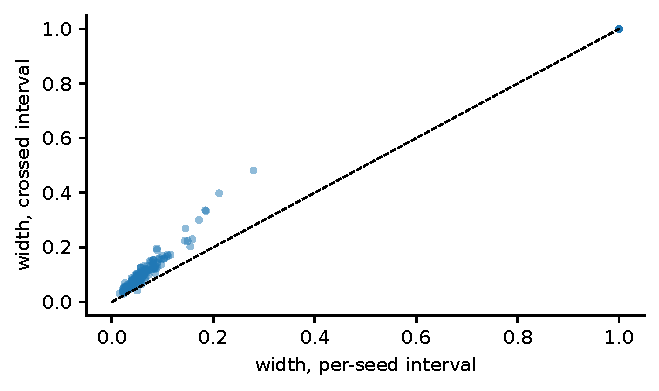
\includegraphics[width=0.52\linewidth]{../stage4_causal_checks/figures/width_scatter.pdf}
\caption{Width of each crossed interval against the per-seed interval of the same contrast (dashed: equal width).}
\label{s4:fig:width}\end{figure}
\begin{table}[H]\centering\scriptsize
\caption{The analyses of this stage under the per-seed and the crossed estimator (same predictions; baseline arms only).}\label{s4:tab:estcheck}
\begin{tabular}{p{5.0cm}p{1.4cm}p{2.6cm}p{2.6cm}p{2.4cm}}\toprule
Result group & Intervals & Excluded 0 only with the per-seed estimator & Excluded 0 only with the crossed estimator & Median width ratio (crossed / per-seed) \\\midrule
capsule/\allowbreak{}dino518\_emb\_groups & 9 & 0 & 0 & 2.02 \\
capsule/\allowbreak{}dino518\_matched & 5 & 0 & 0 & 1.75 \\
capsule/\allowbreak{}dino518\_matched05 & 5 & 0 & 0 & 1.72 \\
capsule/\allowbreak{}dino518\_repro & 5 & 0 & 0 & 1.50 \\
capsule/\allowbreak{}dino518\_sens\_strictB & 9 & 0 & 0 & 1.66 \\
ovary/\allowbreak{}dino518\_emb\_groups & 9 & 0 & 0 & 1.55 \\
ovary/\allowbreak{}dino518\_matched & 5 & 0 & 0 & 1.51 \\
ovary/\allowbreak{}dino518\_matched05 & 5 & 0 & 0 & 1.52 \\
ovary/\allowbreak{}dino518\_repro & 5 & 0 & 0 & 1.55 \\
ovary/\allowbreak{}dino518\_sens\_px50 & 9 & 0 & 0 & 1.62 \\
ovary/\allowbreak{}dino518\_sens\_strictloc & 9 & 0 & 0 & 1.59 \\
review2/\allowbreak{}transplant & 60 & 1 & 0 & 1.63 \\
spec\_e13/\allowbreak{}dino518\_matched & 9 & 0 & 0 & 1.65 \\
spec\_e13/\allowbreak{}dino518\_matched05 & 9 & 1 & 0 & 1.63 \\
spec\_e13/\allowbreak{}dino518\_repro & 9 & 0 & 0 & 1.71 \\
thyroid/\allowbreak{}dino518\_emb\_groups & 9 & 0 & 0 & 1.56 \\
thyroid/\allowbreak{}dino518\_matched & 5 & 0 & 0 & 1.67 \\
thyroid/\allowbreak{}dino518\_matched05 & 5 & 0 & 0 & 1.69 \\
thyroid/\allowbreak{}dino518\_repro & 5 & 0 & 0 & 1.76 \\
thyroid/\allowbreak{}dino518\_sens\_px50 & 9 & 0 & 0 & 1.58 \\
thyroid/\allowbreak{}dino518\_sens\_strictloc & 9 & 1 & 0 & 1.63 \\
\textbf{all} & 204 & 3 & 0 & 1.63 \\
\bottomrule\end{tabular}
\end{table}

\begin{table}[H]\centering\scriptsize
\caption{Contrasts of this stage whose verdict depends on the estimator.}\label{s4:tab:estchanges}
\begin{tabular}{p{4.2cm}p{5.2cm}p{3.3cm}p{2.6cm}}\toprule
Result & Contrast & Crossed estimate [95\% CI] & Verdict vs per-seed estimator \\\midrule
thyroid/\allowbreak{}dino518\_sens\_strictloc & trapB /\allowbreak{} balanced /\allowbreak{} clean /\allowbreak{} balanced /\allowbreak{} erm & $+0.043$ [$-0.008, +0.091$] & no longer excludes 0 \\
spec\_e13/\allowbreak{}dino518\_matched05 & trapA /\allowbreak{} mask /\allowbreak{} clean /\allowbreak{} all /\allowbreak{} mask /\allowbreak{} erm & $-0.026$ [$-0.053, +0.000$] & no longer excludes 0 \\
review2/\allowbreak{}transplant/\allowbreak{}ovary\_dino518 & 0.0 /\allowbreak{} balanced /\allowbreak{} erm /\allowbreak{} test\_rev & $+0.019$ [$-0.006, +0.046$] & no longer excludes 0 \\
\bottomrule\end{tabular}
\end{table}


\subsection{What failed or changed}
\begin{itemize}[leftmargin=*]\itemsep1pt
\item \textbf{The transplant is mostly a paste effect.} The neutral paste reproduces 52--92\% of the interaction; by the
registered rule the transplant is not attributable to the artifact alone in any cohort. No harm figure from the
transplant is attributed to real artifacts.
\item \textbf{Capsule cannot be matched} under the registered rule; its real-trap crossover is descriptive, and its
location evidence rests on the transplant.
\item \textbf{Stricter matching does not improve within-label balance} (up to 0.18--0.19) and shrinks the crossover by
9--16\%.
\item \textbf{The capsule strict-Trap-B variant} gives a smaller crossover, contrary to the expectation registered with it.
\end{itemize}

\subsection{Anticipated questions}
\paragraph{Why not simply adjust for lesion size in the original traps?} Adjustment without matching extrapolates
where the traps do not overlap (hair SMD above 2); matching first restricts the comparison to images that exist in both
traps, and regression then removes what imbalance remains. Doing both is doubly robust: either step alone being correct
is enough.
\paragraph{Why placement values?} AUROC is not a sum over images, so it cannot be regressed directly. Placement values
decompose it exactly into per-image contributions whose class means reproduce the AUROC, so a regression on them adjusts
the crossover itself.
\paragraph{Why is capsule infeasible?} In-ROI debris goes with large lesion boxes (SMD 2.6); among polyp-like lesions
only 19 matched pairs exist, below the registered minimum of 30.
\paragraph{If a neutral paste gives most of the effect, is the transplant useless?} No. It answers the question it was
designed for --- whether the location effect exists on fixed images --- and the neutral paste answers a second question:
the effect is about \emph{any} label-correlated pattern inside the ROI, of which a real artifact is one example. What it
cannot give is an estimate of harm for a particular real artifact.
\paragraph{Why does the neutral paste become a shortcut?} Because the environments make its presence label-correlated,
and a pasted patch leaves a visible seam and occludes the tissue beneath; the encoder can detect both.
\paragraph{Could unmeasured confounding still explain the real-trap crossover?} In principle, yes; matching and
regression only handle measured covariates. The transplant shows that location alone produces the effect on fixed
images, which makes an unmeasured-confounder explanation unnecessary, but it cannot rule one out for the natural traps.
\paragraph{Why group by embeddings rather than ask for patient identifiers?} The data providers do not publish them.
Embedding groups are the strictest available proxy; they reduced thyroid groups from 3,455 to 3,081 without changing the
result.
\paragraph{Why rebuild everything instead of re-running the models?} Re-running on cached objects tests only the last
step. Rebuilding tests the whole chain --- downloads, masks, detectors, groups, features --- and found two gaps in the
reproduction recipe, which were fixed.

\subsection{Conclusion}
\textbf{Supported.} The real-artifact crossover is not explained by measured covariates: it survives matching (3 of 3
feasible cohorts) and doubly robust adjustment (\sFourNATwoOK{} of \sFourNATwo, Holm). Moving the same real artifact inside
the ROI of fixed images reproduces the location effect in all four cohorts, and for hair and thyroid calipers the
artifact's content adds to the effect of the paste. The crossover is robust to the artifact-label definition, to stricter
leakage groups and to a full rebuild. \textbf{Qualified.} Most of the transplant interaction is produced by the paste
itself; unmeasured confounding of the natural location cannot be excluded; capsule is descriptive.
\textbf{Not supported.} A harm figure for real artifacts from the transplant; the capsule matched analysis.

\subsection{Questions for the supervisor}
\begin{enumerate}\itemsep1pt
\item Is matching plus doubly robust adjustment plus the transplant sufficient causal evidence for the thesis, or should a
negative-control analysis be attempted as well?
\item How should the paste effect be presented: as a limitation of the transplant, or as a finding in itself (any
label-correlated pattern inside the ROI defeats masking)?
\item Should capsule endoscopy remain a primary cohort given that its real-trap crossover is descriptive?
\item Is the embedding-group analysis an acceptable answer to the absence of patient identifiers, or must the
limitation be stated more strongly?
\end{enumerate}

